\documentclass[10pt,a4paper]{article}
\usepackage[utf8]{inputenc}
\usepackage{amsmath}
\usepackage{amsfonts}
\usepackage{amssymb}
\usepackage{xcolor}
\usepackage{natbib}
\usepackage{graphicx}
%\usepackage[left=1cm,right=1cm,top=1cm,bottom=1.5cm]{geometry}
\usepackage{geometry}
\author{L\'eo Guignard}
\title{Puck alignment and interpolation}

\DeclareMathOperator*{\argmax}{arg\,max}

\begin{document}
\maketitle
\paragraph{}When doing spatial single-cell transcriptomics, beads are recorded from pucks.
Beads are placed on a 2D matrix where each bead is spaced by a given distance $x_{res}$ (resp.
$y_{res}$) along the $x$ (resp.
$y$) dimension (in our case $x_{res}=y_{res}=6 \mu m$).
These distances define the $xy$ resolution (or lateral resolution) of the slice or puck.
Then, consecutive pucks are spaced by a given distance $z_{res}$ defining the $z$ resolution (or axial resolution) of the dataset (in our case $z_{res}=30\mu m$).
\paragraph{}Because the pucks are physically moved between their slicing and their acquisition, they are not acquired within the same frame (meaning that they are not aligned).
In order to reconstruct a 3D representation of the single cell transcriptomics of the acquired embryo and to do full 3D spatial analysis, it is necessary to align consecutive pucks to recover the spatial integrity of the specimen.
Moreover, because the axial resolution is significantly greater than the lateral one, in some cases, it is necessary to interpolate the data between the pucks.
\paragraph{}In the following section we will describe how this alignment was performed together with how the beads were interpolated between pucks.
\section{Notation}
\paragraph{}We define our dataset as a set of pucks \(\mathcal{P}=\{P_i\}\).
The function $c_P$ maps a puck to its height coordinate $z_i$: \(c_P: P_i\in \mathcal{P} \rightarrow z_i \in \mathbb{R}\).
Each puck $P_i$ is itself a set of beads, \(P_i=\{b_{ij}\}\) and similarly to the pucks, the function \(c_b\) maps a bead \(b_{ij}\) to its \(xy\) coordinate within the puck: \(c_b:b_{ij}\in P_i\rightarrow (x,y)\in \mathbb{R}^2\).
From \(c_P\) and \(c_b\) we define the function \(c:b_{ij}\in P_i\rightarrow (x,y,z)\in\mathbb{R}\) which maps a bead to its 3D spatial coordinate.
Note that \(c_P\) defines a total order on the pucks.
Let then \(\mathcal{P}\) be ordered such that \(\forall i,j,~P_i<P_j\iff c_P(P_i)<c_P(P_j)\).
%%
\paragraph{}Moreover, using the previously described analysis, we can associate each bead to the tissue it most likely belongs to, the function \(T:b_{ij}\in P_i\rightarrow t\in\mathcal{T}\) where \(t\in\mathcal{T}\) maps each bead to a unique identifier for the tissue it belongs to. \(\mathcal{T}\) is the set of possible tissues previously identified.
Similarly, to each bead is associated a value for each given gene analysed in the dataset.
This value is correlated to the level of expression of said gene for said bead.
Given a gene \(g\), we define the function \(E_g:b_{ij}\in P_i\rightarrow e\in\mathbb{R}\) which maps the value \(e\) of expression of the gene \(g\) to the bead \(b_{ij}\).
%%
\section{Pre-processing}
\subsection{Removing the remaining outliers}
\paragraph{}Before aligning the pucks it is possible to remove beads that are likely to be noise.
Within a given tissue, noisy beads were detected as the beads that were spatially further away from their neighbors than the normal distribution of the spatial distances between beads.
To assess the normal distribution of spatial distances between beads of a given tissue, we first computed the distance between any given bead and its closest bead from the same tissue type.
We then analysed the distribution of these distances by fitting a gaussian mixture model, with a number of components equal to \(n_{components}\) (in our case we used \(n_{components}=3\).
When using 3 components, the \(1^{st}\) and \(2^{nd}\) components are assumed to be real.
The \(3^{rd}\) component, with the higher mean, is the distribution of distances of noisy beads.
We then discarded all the beads that had a distance to their closest neighbor from the same tissue which had a probability to belong to the first or second component were lower than \(th_{gmm}\) (in our case we used \(th_{gmm}=0.6\%\)).
This pre-processing step is not mandatory but it can help getting more accurate results. The value might vary depending on the sample and tissue analyzed.
\section{Aligning the pucks}
\paragraph{}As previously mentioned, due to the nature of the acquisition process, consecutive pucks do not live within the same frame.
They are therefore not spatially comparable.
\paragraph{}To align the pucks and register them onto the same frame, we first chose our first puck in \(\mathcal{P}\), \(P_0\), as the reference puck.
We then registered each following slide to its preceding one: \(P_1\) is registered onto \(P_0\), \(P_{i+1}\) is registered onto \(P_{i}\) and so on and so forth.
Ultimately we can compose all the transformations together to register any puck onto the first puck.
To compute the transformation necessary to register two consecutive pucks, we first performed a coarse grain alignment using the center of mass of a subset of the different tissue types.
We then refined the alignment by pairing beads across the pucks and by aligning them.
\subsection{Coarse grain alignment}
\paragraph{}We first chose a subset of tissues \(\mathcal{L}\subset\mathcal{T}\) that are spatially localised (for example heart tube precursor beads or somite precursor beads).
We then discarded (only for the coarse grain alignment) tissues that were spread in space (for example blood precursor beads).
An exhaustive list of the discarded tissue types can be found below.
\paragraph{}Then we computed the alignment transformation (\(r_{i\leftarrow j}^*\), registering the puck \(P_j\) onto the puck \(P_i\)) as the rigid transformation (translation plus rotation) that minimizes the sum of the squared distances between corresponding tissue types center of mass:
\begin{eqnarray}\label{eq:rigid}
r_{i\leftarrow j}^*&=&\argmax_{r\in\mathcal{R}} \big\{\sum_{t\in \mathcal{L}}||COM_i(t)-r[COM_j(t)]||_2\big\}
\end{eqnarray}
where \(COM_i(t)\) is the position of the center of mass of the tissue \(t\) in the puck \(i\), \(||\cdot||_2\) is the L2 norm and \(\mathcal{R}\) is the set of all rigid transformations.
\(r[COM_j(t)]\) is therefore the position of the center of mass of the tissue \(t\) in the puck \(j\) after application of the rigid transformation \(r\).
\paragraph{}We then applied the composition of the necessary transformations to register all pucks onto the first puck.
For example, to register the puck \(j\) onto the puck \(0\), we applied the transformation \(r_{0\leftarrow j}^*=r_{0\leftarrow 1}^*\circ r_{1\leftarrow 2}^*\circ \cdots \circ r_{j-1\leftarrow j}^*\).
\subsection{Alignment refinement}\label{subsec:ali-ref}
\paragraph{}To refine the alignment, we then paired beads from consecutive pucks.
Only beads from the same tissue types could be paired.
The pairing was the one that minimizes the sum of the distances between paired beads (using the solution of the linear sum assignment optimization).
The distances were computed after applying the coarse grain transformation.
From this pairing, as previously, we computed the rigid transformation \(R^*_{i\leftarrow j}\) that minimizes the sum of the squares of the distances between the paired beads (see eq.\eqref{eq:rigid}).
\section{In between puck interpolation}
\paragraph{}As shown earlier, the distance between two consecutive beads within the same puck is significantly smaller than the one between two pucks (one order of magnitude in our case, 6\(\mu m\) versus 30\(\mu m\)). This property makes it that some analysis of the 3D volume of the embryo is difficult or even not possible. If one wants to study a plane that is tilted by a small angle to the original puck planes, the beads become too scarce. To overcome this issue, we designed an algorithm to interpolate beads in between pucks. The goal is to create beads where there would likely be and to assign to these interpolated beads gene expression values that are the most likely values.
\paragraph{}To interpolate beads between pucks, we first paired beads belonging to the same tissues (similarly to the pairing that was done in \ref{subsec:ali-ref}) to construct paths of beads (see Fig. \ref{fig:interp} A-B). We then assume a smooth continuity of gene expression and position to compute the interpolation. This smooth and continuous hypothesis on the system is the basis of the interpolation. It is important to keep this hypothesis in mind when doing any further analysis since it might not apply to all samples or tissue types.
\subsection{Bead pairings and paths}
\paragraph{}The first step towards in-between puck interpolation is to build a path of beads from consecutive pucks.
These paths were built by pairing beads from consecutive pucks.
Beads were paired based on their spatial proximity.
As previously, we used a linear assignment algorithm to pair beads.
Linear sum alignment requires that a positive cost is computed between any beads that can be paired together.
Here, we used as our cost function the Euclidean distance (hence the spatial proximity bead pairing).
The bead pairing between consecutive pucks creates paths of beads. A path of beads is a series of beads that are paired sequentially by the puck to puck pairing.
For example \(b_{i,j}\) is paired to \(b_{i+1,k}\) which is paired to \(b_{i+2,l}\). These paired beads then create the path \(Pa_{i,j}=(b_{i,j}, b_{i+1,k},b_{i+2,l})\).
\paragraph{}Because each path does not start (resp. end) at the first (reps. last) puck of the sample, to avoid abrupt and artificial stops of the paths, we computed intermediate beads which would mark the most likely end of the path (see Fig. \ref{fig:interp} C). The position of these beads added in between pucks (let them be \(b^{proj}_{i,j}\)) was computed as follow:
\begin{equation}\label{eq:proj}
c(b^{proj}_{i,j})=c({b_{i,j}})+\frac{n}{|\mathcal{N}^p_{i,j}|}\sum_{b_{i,k}\in \mathcal{N}^p_{i,j}}\overrightarrow{b_{i,k},p(b_{i,k})}
\end{equation}
where \(p(b_{i,k})\) is the projection of \(b_{i,k}\) in the following puck. \(\mathcal{N}_{i,j}\) is the set of beads that are neighbors of \(b_{i,j}\) according to the Gabriel graph tessellation of the set of beads for a given puck.
\(\mathcal{N} ^p_{i,j}\subset \mathcal{N}_{i,j}\) is the subset of neighbors of the bead \(b_{i,j}\) that have a projection, meaning that \(p(b_{i,j})\) exists.
\(n\) is the fraction of the average projection to consider. \(n\) is computed with regard to the distance of the bead \(b_{i,j}\) to its closest neighbor that has a projection.
The closer a bead is to a bead with a projection, the larger \(n\) will be, meaning that if a bead is close to a bead that is linked to another bead in the following puck, the longer it will exist in between the pucks.
Note that the Gabriel graph tessellation is a decimation of the more classical vorono\"i tessellation which avoids most of the usual issues of the vorono\"i tessellation especially when it comes to concave set of positions (see \cite{mcdole:2018}).
\begin{figure}
\center
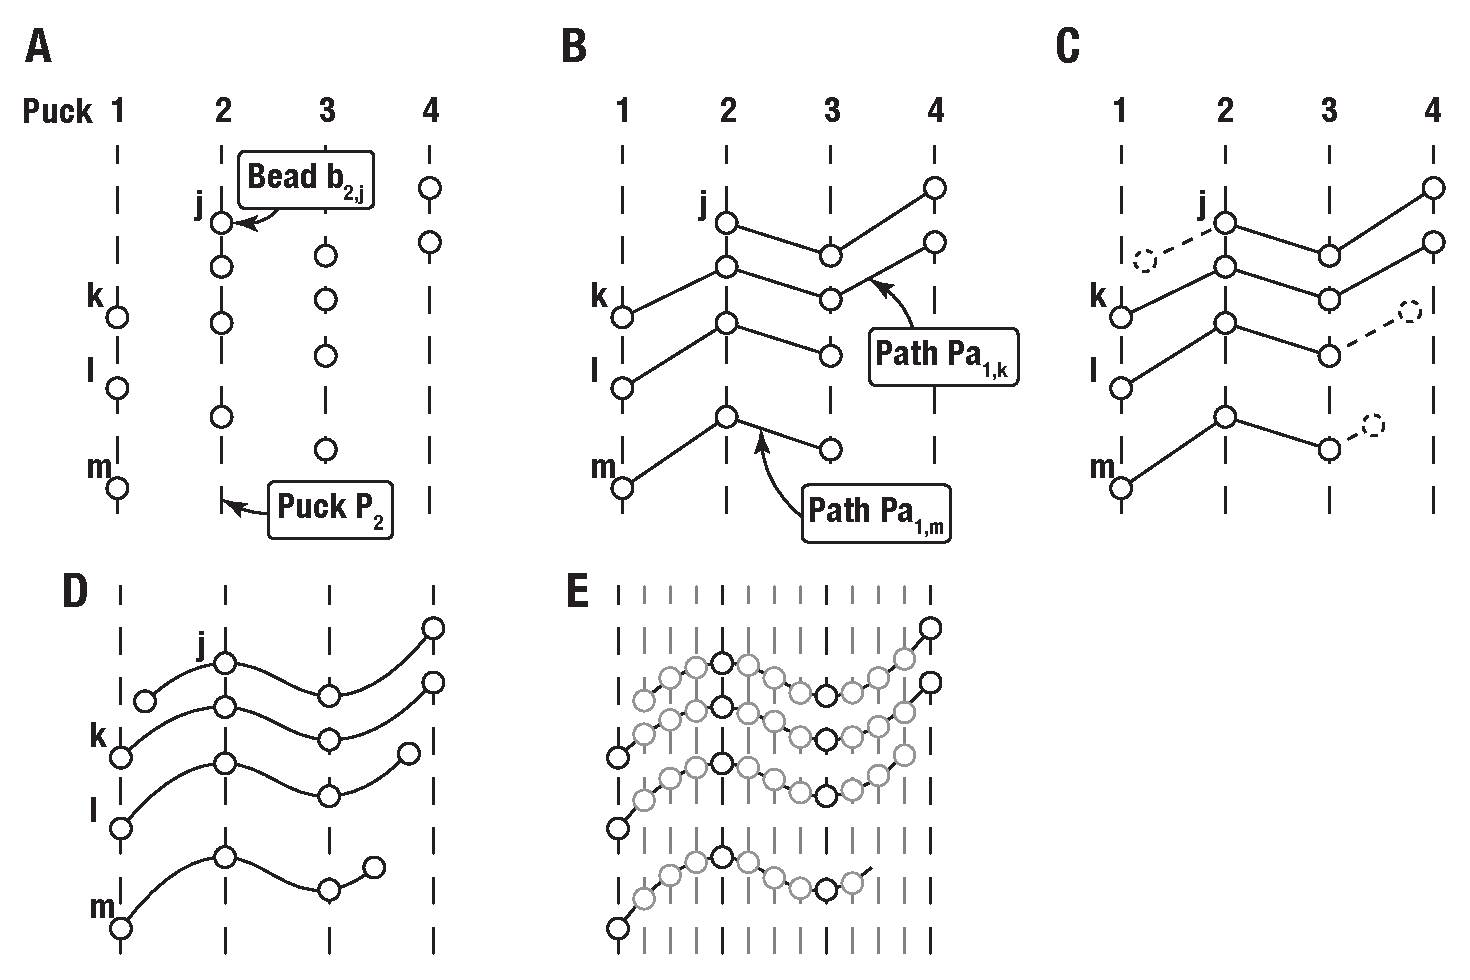
\includegraphics[width=0.8\textwidth]{figures/interpolation}
\caption{\textbf{Schematics of inter puck bead interpolation.} A. Schematics of original data. Dashed lines represent the pucks, circles represent the beads. B. Pairing between beads of consecutive pucks forming the different paths. C. When necessary, addition of the in-between puck projections. D. Resulting splines from the bead paring. E. Interpolation of beads in between the pucks, the grey beads are the interpolated ones.}\label{fig:interp}
\end{figure}
\subsection{Interpolation from the paths}
\paragraph{}Once the paths are created, all existing beads belong to a single path.
From these paths, positions and gene expressions can be interpolated.
Here, we interpolated the positions and gene expressions in between pucks as univariate cubic splines. Therefore, it is possible to retrieve the set of beads that live at any given \(z\) position together with the interpolated gene expression (see Fig. \ref{fig:interp} D-E).
\section{Spatial differential expression}
\paragraph{}The goal here is to score genes on whether they are locally expressed or not.
To do so we used the fact that given a set of points and their positions in space, if some points are randomly removed independently of their positions, the resulting number of remaining points is linearly correlated to the average remaining number of neighbors for each remaining point.

In other words, the previous paragraph means that if beads are randomly expressing a given gene in space (as opposed to locally/differentially), the volume of expressing beads is linearly correlated to the average density of expressing beads.
\paragraph{}We then computed the expression threshold above which a bead is considered expressing.
The threshold was computed independently for each gene-tissue pair as the value that split the distribution of expression values for each gene within each tissue into two classes. For that we used the Otsu method \citep{Otsu:1979} which splits a distribution into two such that the intra-class variance is minimum (and therefore maximizing the inter-class variance).
\paragraph{}Having split the beads into two separate classes, the expressing and non-expressing beads, we then compute the volume of expressing beads (number of positive beads) and the average local density (average number of expressing neighbors). These two values are then normalized by the total volume and the average number of neighbors of each bead respectively.
\paragraph{}We assumed that most genes are either ubiquitously expressing or not expressing at all within a given tissue.
Their thresholding then results in a random spatial distribution of positive and negative beads laying the ground for computing the linear relationship between volume and density for each given tissue.
For each gene, the distance to the linear regression is then calculated which is the score for spatially expressed genes.
\bibliographystyle{apalike}
\bibliography{references}
\end{document}